\chapter{Answering questions with astronomical images}

Last week, you learned how we use lenses and telescopes to bend light. This week, you will analyze images that were taken by a research-grade robotic telescope, learn how we record these images, and learn one way to analyze those images to create knowledge about the distance between stars.

%Last week, you queued up some images to be taken by the robotic telescope and learned how telescopes work to create images. This week, you'll learn how we record these images, and you'll learn one way to analyze those images to create knowledge about the distance between stars.

\section{Learning goals}

\begin{itemize}
	\item Answer questions by analyzing data that you took yourself.
	
	\item Experience and analyze the light gathering and angular resolution benefits of telescopes.
	
	\item Use pixel scale and length measurements to determine the angular separation of objects in a digital image.
	
%	\item Gain insight of and appreciation for the scale of astronomical distances.
\end{itemize}

\subsection{Other skills learned}
\begin{itemize}
	\item Calculate pixel scale, plate scale from an image of known objects
	\item Measure distances with DS9
	\item Convert between angular separation and length
	\item Use trig functions with triangles for the above conversion
\end{itemize}

\section{Lab Team Roles}

Decide which team members will hold each role this week: facilitator, scribe, technician, skeptic. If there are three members, consider distributing the first three roles, then adding the skeptic role to someone as a second role.

\section{Telescopes and angular size}

To gain some intuition for the functions of telescopes and for the concept of angular size, \textbf{complete the worksheets on the next 4 pages}. For ease, you can answer them in your lab report instead of drawing right on them, if you'd like.

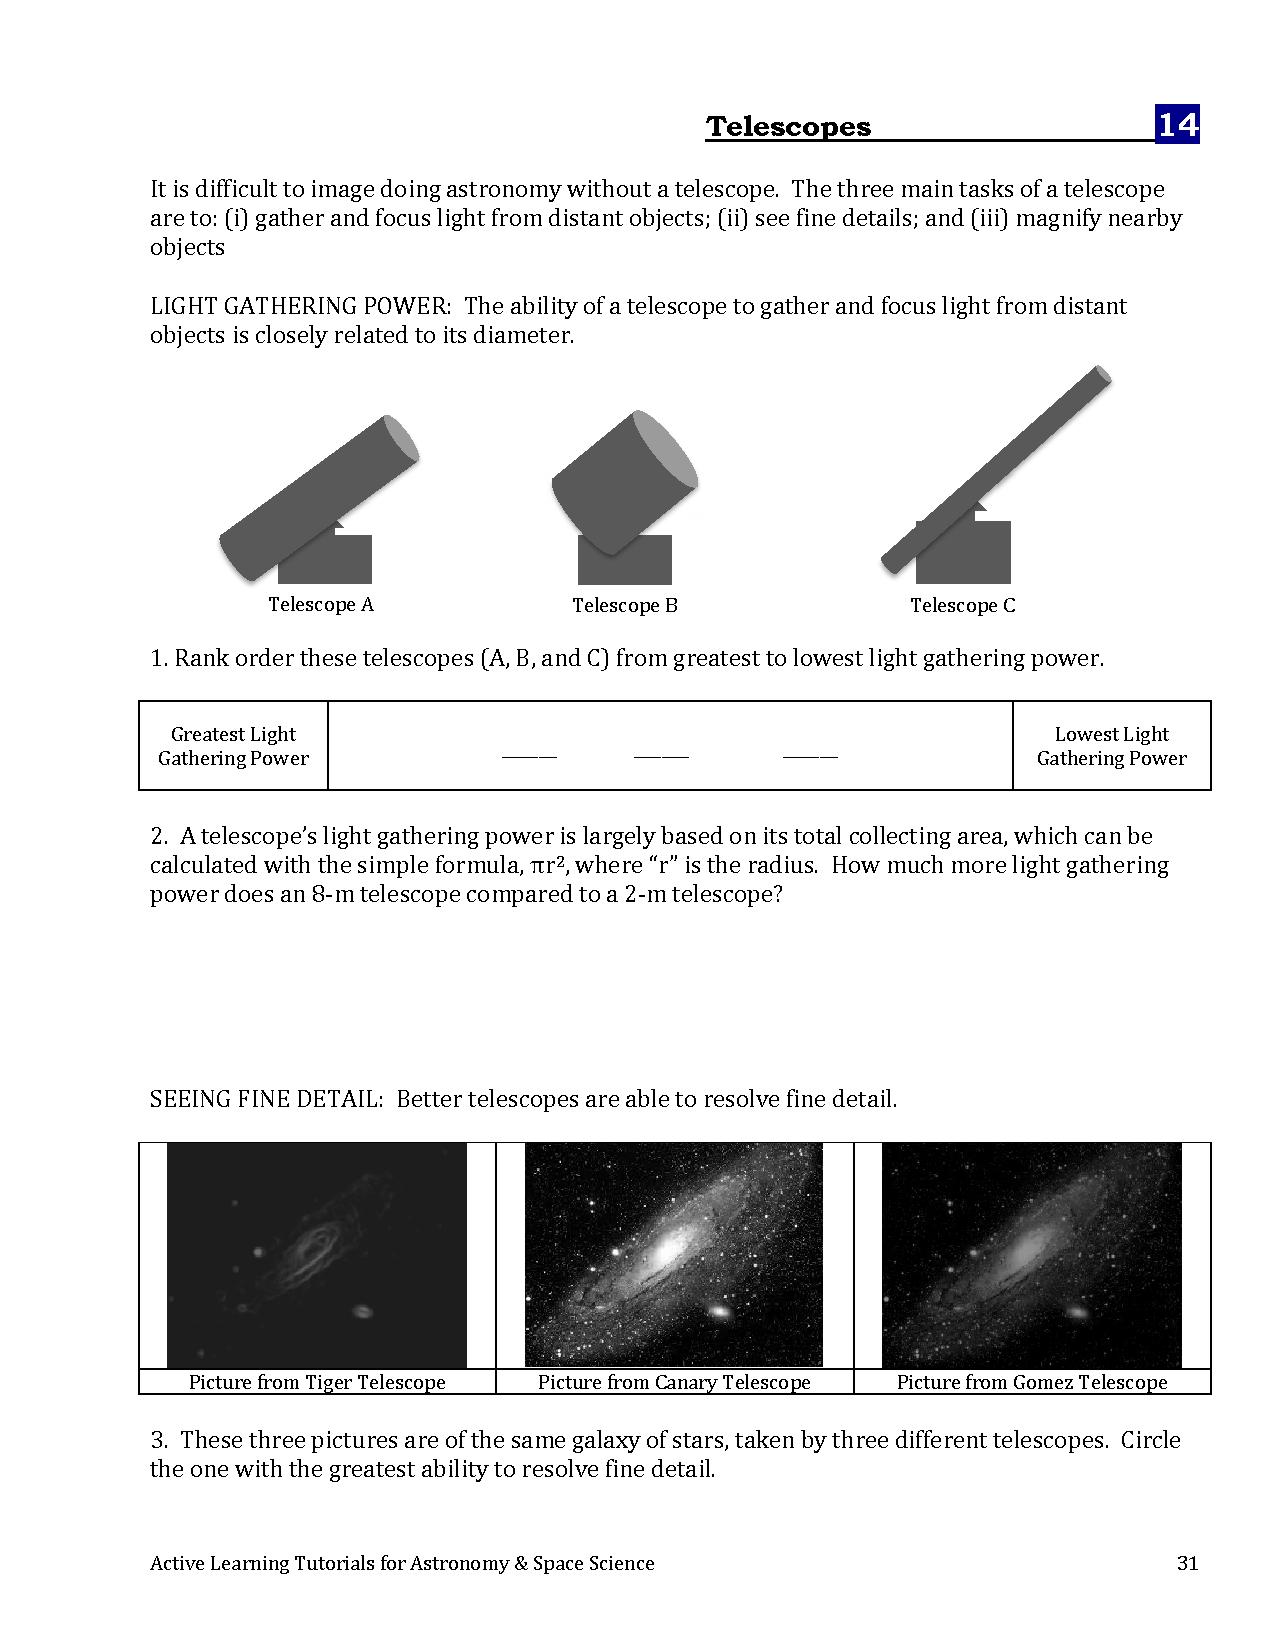
\includepdf[pages={-}]{astro-images-remote/ALT-ASS-Astro-telescopes-angular-res.pdf}

\section{How big is your face?}

This is a simple question, so that you can learn some astronomical concepts and tools while answering it and still keeping the subject matter intuitive.

\subsection{Background: reflecting telescopes and CCDs}

The primary utility of a telescope is its ability to gather light, thereby enabling visualization and analysis of the faint astronomical objects we are trying to observe. This requires focusing light incident on a large surface area. We will be using a \textbf{reflecting} telescope, which means that light rays from observation targets are focused into an eyepiece or onto a detector with reflecting mirrors. This is in contrast to refracting telescopes, which use refracting lenses to focus light rays. Figure~\ref{sot:fig:schmidt} shows schematically how this kind of telescope works. 

\begin{figure}
	\centering
	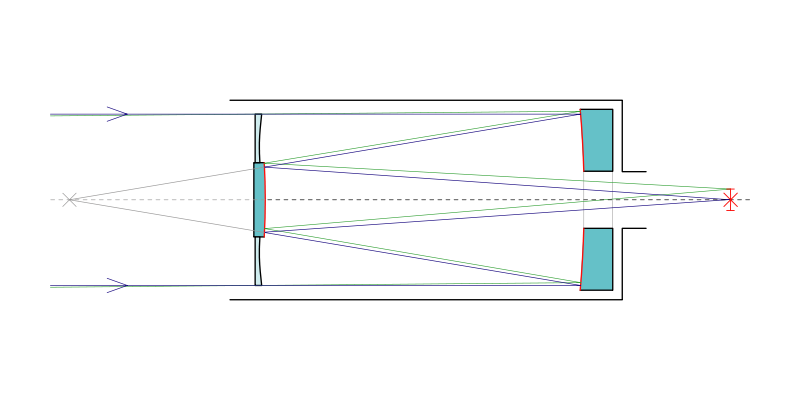
\includegraphics[scale = 0.5]{small-optical-telescopes/Schmidt-Cassegrain-Telescope.png}
	\caption{Schematic for a reflecting telescope of a Schmidt-Cassegrain design. 
		Light rays from astronomical objects enter the telescope in parallel because their source is effectively at infinity. They are then reflected by a parabolic primary mirror onto a secondary mirror that again reflects the light to a focus. An eyepiece or a camera is placed at the focal plane of the resulting image. Image source: \url{https://en.wikipedia.org/wiki/Cassegrain\_reflector\#/media/File:Schmidt-Cassegrain-Telescope.svg}}\label{sot:fig:schmidt}
\end{figure}

%To take images in this lab, and to observe astronomical objects using the SEO, we make use of a \textbf{Charge Coupled Device (CCD)}.
To take images during this lab with your smartphone or digital camera, and for the images taken by the Stone Edge Observatory telescope, we make use of a \textbf{Charge Coupled Device (CCD)}.
CCDs are the standard detectors for taking astronomical images at wavelengths blueward of (lower wavelength than) approximately 1 micron. Think of the observatory's CCD a
very advanced low-noise digital detector, not wholly dissimilar from the digital detector in your
smartphone. Every time a photon within a certain energy range hits the detector, an electron is knocked off of the incident pixel, charging that pixel's capacitor. Thus, for each pixel, more photons $\implies$ more electrons $\implies$ more charge, and the charge can be read off into a digital signal that is then processed as an image. 

%% Don't need to know the following yet, until we play with color.
%The main thing to note is that the CCD material is not sensitive to all wavelengths of light uniformly. Photons of certain energies are more likely to excite electrons in the detector and thus contribute to the output image. Consequently, the observed image intensity will be weighted by the response function of the detector.

\subsection{Finding your pixel scale}

To find out how big your face is the same way you might find out how big a planet is, you need to know the pixel scale of your camera, which is what angle a single pixel covers (this quantity is also your optical system's maximum angular resolution). A simple way is to take an image of something with known angular size, then divide that by the number of pixels it takes up.

\textbf{Equipment:} Smartphone or digital camera, object of known length, ruler or other method of measuring distance across your room, the software SAOImage DS9.

\begin{steps}
	\item Download and install DS9 from \url{http://ds9.si.edu/site/Download.html}. SAOImage DS9, or DS9 for short, is an image viewer, analyzer, and processor written and used by astronomers for working with astronomical images.
	
	If you click the link to download, it might say "redirecting" while never actually redirecting. In this case, copy the link into the address bar directly.
\begin{framed}	
	\textbf{For MacOS}, unless you know otherwise, choose from the top set of choices (to the right of
	the blue apple logo). To find your version, from the Apple menu in the corner of the screen,
	choose “About This Mac”.
	
	If it displays a warning and prevents you from installed from an unidentified developer, follow the instructions at the following link to create an exception:
	
	\url{https://support.apple.com/guide/mac-help/open-a-mac-app-from-an-unidentified-developer-mh40616/mac}
\end{framed}

	\item Set up an object of known length at a known distance from the camera. For example, US Letter sized paper has a standard size, as does currency. You can measure the distance from the camera with a tape measure or other standardized objects. \textbf{Record a length of the object and the distance to the camera, including uncertainty.} Discuss with your group how to estimate the measurement uncertainty.
	
	\item Calculate the angular size of the object and propagate the uncertainty (see Appendix \ref{unc:sec:prop}) from the two measured quantities to report the angular size in the format $A \pm \delta A$.

	To find the angular size of the object, as seen by the camera, you can use the formula
	\begin{equation}
	 \tan \theta = \frac{\textrm{physical size}}{\textrm{distance}}\,.
	\end{equation}
	For situations where the object is far away compared to its size ($\gtrsim 5$ times more distant), you can apply the small-angle approximation, where $\tan \theta \approx \theta$, to simplify the formula to
	\begin{equation}
	 \theta = \frac{\textrm{physical size}}{\textrm{distance}}\,.
	\end{equation}
	Note that the resulting angle will be in radians, not degrees.

\begin{figure}
	\centering
	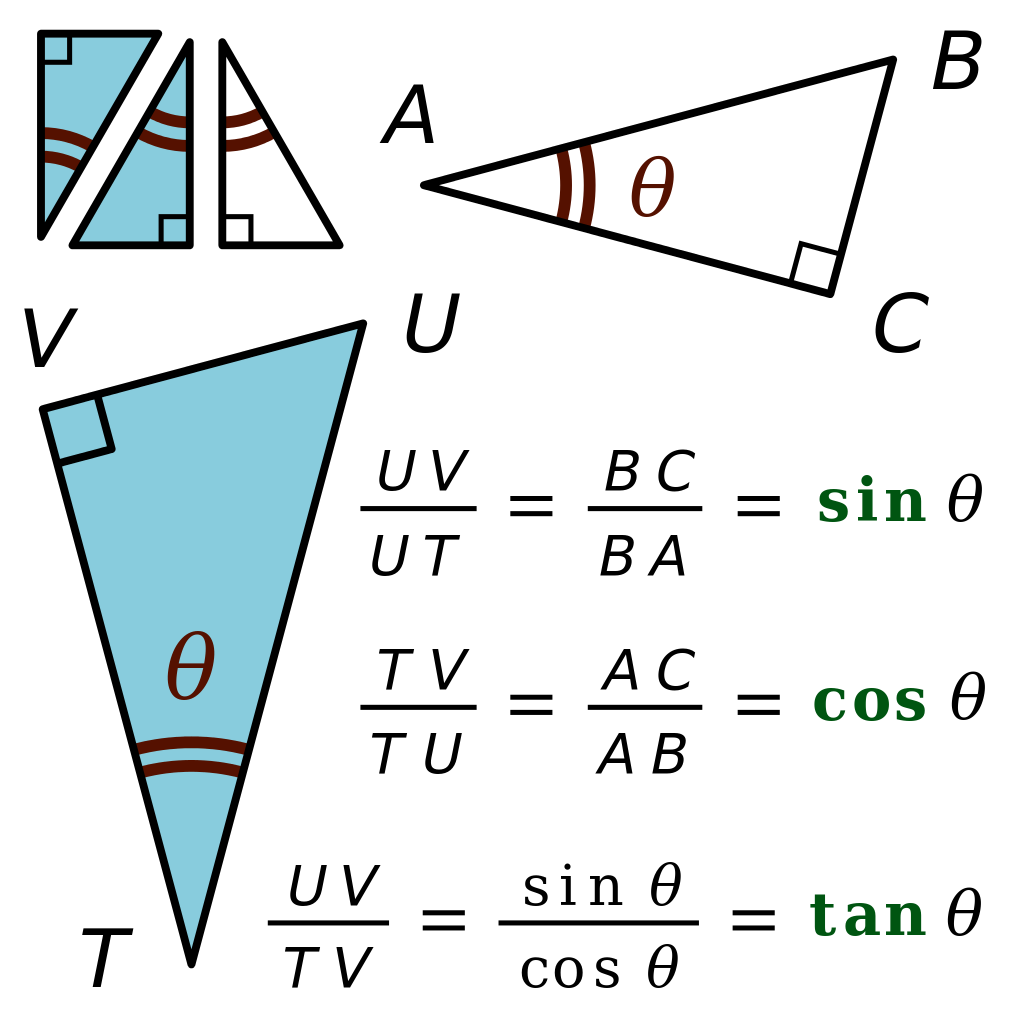
\includegraphics[width=0.35\textwidth]{astro-images-remote/1024px-Academ_Base_of_trigonometry_svg.png}
	\caption{Trigonometric relations for triangles. ``UV'' is the distance between vertices U and V. (Image by \url{https://commons.wikimedia.org/wiki/User:Baelde})}\label{ai:fig:trig}
\end{figure}

	\item Take an image of the object with your camera and copy it to the computer that has DS9 installed on it. \textbf{Include this image in your lab report and label the known object.}
	
	\item The standard image format for astronomical images is FITS. Convert your image to the FITS format at \url{https://www.online-utility.org/image/convert/to/FITS}
	
	\item Open the FITS file in DS9.

\end{steps}
	
	Notice that the image displays in grayscale, and their is another window that opens titled ``Cube'', that has a slider in it. When you move the slider, the image will change slightly. What is happen is that a CCD pixel, by itself, does not know the wavelength of the photon (and thus the color) that it receives. To resolve color, a color filter is placed over the pixel. In consumer cameras, red, green, and blue color filters are attached permanently over different pixels, in a pattern so that all parts of the CCD have equal coverage of the different colors. DS9 reads this and separates the three filters so that each color filter band can be analyzed separately.
	
\begin{steps}
	
	\item Measure the length of the known object in pixels using DS9. There are two ways to do this:
	\begin{enumerate}
		\item One is to place the cursor at each end of the object, record the x and y pixel coordinates at each end, and find the straight-line distance between them (find the x difference and y difference, then use those in Pythagorean's theorem to find the hypotenuse).
		
		\item The other way is to use the ruler tool. To measure a length, select Region $>$ Shape $>$ Ruler from the drop-down menu. Then select Edit $>$ Region. Now if you click and drag on the image, it will draw a line and display the distance in pixels, or in angular separation if the image file has been calibrated withe pixel scale already.
	\end{enumerate}
	
	\textbf{Record the length in pixels and your estimated uncertainty.} To get the uncertainty, you can try doing the above measurement several times and calculate the mean value and the uncertainty of the mean (see Appendix \ref{unc:random}). 
	
	\item Calculate the pixel scale, which is the angular range that each pixel sees. Express it in units of degrees (or arcminutes or arcseconds) per pixel. Find the uncertainty by propagating the uncertainties. \textbf{Record the pixel scale of your camera}.

	\item Based on the pixel scale alone, how far apart in angle would two stars need to be in order to be distinguished as two objects instead of one?

\end{steps}

\subsection{Measuring your face}

Now that you have the pixel scale, you can image another object and find its angular size. And if you know the distance to it, you can find its physical size.

\begin{steps}
	\item Now take a selfie.
	
	\item Use the pixel scale that you determined, along with that image, to find the angular separation between two points in the image --- for example, what is the angle subtended by your eye? Use the distance from the camera to the person to also determine the distance between those two points, for example in millimeters.
	
	\item Estimate the uncertainty, and \textbf{record the angular separation, physical size, and uncertainties for each}.
\end{steps}

%\subsection{Telescope Set Up, Preliminary Observations}\label{ai:sec:setup}
%
%The telescope and camera assembly is an expensive and relatively fragile piece of hardware, so
%move carefully when interacting with the system. We have only two setups, so the class will be split into two groups for using the classroom telescope.
%
%First we will be observing an object at the opposite end of the lab room with the lights turned off. During this exercise we will 1) check that the telescope is focused (which should already be the case), 2) gain practice positioning the telescope and targets, and 3) demonstrate the light gathering and angular resolution capabilities of the telescope with a physical object for which you have an direct sense of scale. \textbf{NOTE: For safety purposes, do not walk around the
%	lab while the lights are off; instead, turn the lights off only as needed to gather data
%	or make observations, and when the lights are off, don’t move about significantly.}
%
%\begin{steps}
%	\item The telescope should already be set up, with the camera on and cooled, and be approximately
%	in focus and pointed at the target at the other end of the lab bench. If not, your TA will
%	work with you to get the setup roughly correct.
%	
%	\item Your first task will be to tweak the centering of the image target. This doesn’t have to be
%	perfect, but you should be able to see the mm scale marks. The telescope can be moved in elevation (up-down). The fine control of elevation is achieved using a knob on the mount - your TA will show you details. To shift the image left or right, move the target instead.
%	
%	\item Next we want to precisely focus the telescope. Do this with most of the lights off --- otherwise
%	the image has too much light. Use the 4th filter of the five available; this can be selected
%	from the ‘Filter’ menu. Then, use the \textbf{Focus} task from the camera control system toolbar,
%	and take images of a few seconds (at most). If the image is completely dark, and the peak intensity number in the focus box is reading around 65000, then the CCD is saturated, and the light in the room should be reduced, or the exposure time shortened.
%	
%	\item Start the focus sequence - the camera will just
%	take and display images repeatedly, of the exposure duration you specified. Now, adjust
%	the focus knob (on the back of the telescope, off center) until you achieve an optimal focus.
%	Note that you can (and should) zoom the magnification of the image so you can see the
%	imaging target in detail. Do this by adjusting the magnification, and adjusting the image
%	x,y centering so you’re looking at an appropriate zoomed location in the image. Note that
%	you’ll need to not be touching the telescope or mount to get a sharp image, so you’ll
%	have to adjust, then move away, wait, and repeat. Your classmates walking around the lab
%	will cause image shake that will make focusing difficult, so enforce a still classroom while
%	you do this.
%
%	\item Once the telescope is focused, \textbf{grab a 1-second exposure} using the Grab command.
%	
%%	\item Time to demonstrate one helpful aspect of telescopes by taking an image in the dark. Once the telescope is focused to the sharpest possible images, turn off the lights and acquire an image using the
%%	\textbf{Grab} button on the toolbar. An exposure time of 40--60 seconds is usually good with all of
%%	the lab lights off and the blinds closed.
%	
%	\item Save this image in ‘fits’ format; the ‘ds9’ tool available on all of the lab
%	computers can be used to examine the image in detail (you can also install this free software on your computer). You can use the university supported
%	’Box’ system to share data with your lab classmates (or any other filesharing app that you prefer). See \url{uchicago.account.box.com/login}
%	for details.
%	
%%	\item With the lights back on, gather around the target on the lab bench and then
%%	turn the light off again. Observe the target. Can you see it? Can you see the details? Does
%%	it matter how close you are (Rubric Row B5)?
%%	
%%	\item Compute and report the ratio of the light gathering power of
%%	the telescope relative to your eye, and comment on how that relates to what you do (or do
%%	not) observe by eye compared to the telescope (Rubric Row B9).
%
%	\item Load the image in DS9. You can adjust the contrast of the image by holding down the right-click and dragging left, right, up, and down. In the upper right window, you can drag the frame around to view different parts of the image. To measure a length, select Region $>$ Shape $>$ Ruler from the drop-down menu. Then select Edit $>$ Region. Now if you click and drag on the image, it will draw a line and display the distance in pixels, or in angular separation if the image file has been calibrated withe pixel scale already.
%	
%	\item In the acquired and saved image you can see a mm scale, which correponds to some number
%	of pixels. Compute and report the ‘pixel scale’ in mm/pixel. Given the distance between the
%	telescope and the target, what is the angular pixel scale in arcseconds/pixel?
%	
%	To find this, note that for an arc (segment) of a circle, the length of that arc $s$ is related to the radius of circle $r$, and the angle (in radians) subtended by that arc $\theta$ by
%	\begin{equation}
%	s = r \theta
%	\end{equation}
%
%	\item Based on the pixel scale alone, how far apart in angle would two stars need to be in order to be distinguished as two objects instead of one?
%	
%	\item Observe the target from the vantage
%	point of the telescope by eye. What detail can you see? How does that compare to what
%	you can see with the telescope?
%	
%	\item Now take an image of part of one of your groupmates with the telescope. Centering on their eye can make for a fun picture. Use the pixel scale that you determined, along with that image, to find the angular separation (or ``angular distance'') between two points in the image --- for example, what is the angle subtended by their eye? Use the distance from the telescope to the person to also determine the distance between those two points, for example in millimeters. %Estimate your uncertainty and compare this measurement to a direct one (by holding up a ruler, for example.)
%\end{steps}

\section{How far apart are these stars?}

Now that you have experience measuring distances for objects you can directly measure, you'll try your hand at measuring distant objects that none of us can measure directly --- stars that were imaged by our robotic telescope at Stone Edge Observatory.
%other stars in your image from SEO!
The goal here is to pick two stars in your image and find the angular separation between them.
%, as well as physical distance. To get the physical distance, you'll need to know their distances from Earth.
To check your work, you can compare to the known positions of these stars. To get that, you'll need to match up those stars in your image to known stars. You can use Stellarium for this, a free virtual observatory app. Then you can select those stars in the app and easily find information about them.

%Note that since we are using a real robotic telescope, many things can go wrong that may result in you not having an image that you've taken. There could have been cloudy nights all week, or smoke from wildfires, or planned power outages to protect from wildfires, or part of the observatory could have broken down. We have archival images in the case that your images are not taken, so that you can still complete the lab.

\begin{steps}
	\item Download the FITS file for 51 Pegasi from the Labs module in Canvas. 51 Peg is the star system where humans detected our first exoplanet.
	
% Second brightest star is Gaia DR2 2832576492727851136. The angular distance between 51 Peg and that one is 0.159841 deg (9'35.4'')
	
	\item Load the image in DS9. You can adjust the contrast of the image by holding down the right-click and dragging left, right, up, and down. In the upper right window, you can drag the frame around to view different parts of the image.

%	\item Log into \url{queue.stoneedgeobservatory.com}, find your completed observation, and click ``go to image''. If you don't have a completed observation, find a classmate's or TA's image URL to visit to get an image to work with. If the image that appears is very fuzzy or has no stars in it, choose a different option from the ``Pipe Step'' drop-down menu.
	
%	\item Select the link ``Download Selected FITS File'' to do so. Open it in DS9.

	\item Also open \url{stellarium-web.org} and search for 51 Pegasi.
	
%	\item Also open Stellarium on a computer. It is a free open source virtual observatory, so you can install it on your computer if you'd like. Use Stellarium to find your target (hover over the left edge of the screen to find the menu that includes the Search function). Toggle the Ground and Atmosphere in the bottom menu, so you can see the star clearly. Zoom in by selecting the rectangle icon third from the right in the upper-right-hand corner. This simulates a field of view that is similar to our telescope.

	\item The field of view (total angular size of image) for SEO is 27', so zoom in Stellarium to the same approximate field of view.
	
	\item Use the Stellarium and the downloaded image to identify two stars, 51 Peg and one other. Note that the two pictures might be rotated or flipped relative to each other.
	
	\item For those two stars, use DS9 to measure the angular separation (angular distance) between them. You may need to use the pixel scale of the Stone Edge Observatory telescope, which is 0.76''/pix (arcseconds per pixel). \textbf{Record this and your uncertainty for it.}
	
	\item In Stellarium, select each of the two stars in turn and record their equatorial coordinates (RA/Dec). Calculate the angular separation using a web form, for example \url{http://hea.iki.rssi.ru/AZT22/ENG/cgi-bin/c_dist.htm}.
	
	\item Use the $t'$ statistic (see Appendix\ \ref{unc:sec:comparing}) to compare these two values of angular separation.
	
%	\item To find the physical distance between them, use the distances from Earth as given in Stellarium, along with the angular separation and some geometry.
	
%	\item How long does it take light to travel from one of those stars to the other?
\end{steps}

%\section{But wait! Next set of observations with SEO}

%In the next lab, we will be exploring the use of color in astronomical images. The CCD image sensor is monochrome. That is, it has a relatively flat sensitivity to different wavelengths in the visible spectrum. To gain information about color, or the relative contributions of different wavelengths, you'll use filters that can be placed in front of the sensor. So for next week, \textbf{queue another observation or several} (no more than 1 per student per week). Choose the same target from last week. Select the r, g, and b filters (red, green, and blue, respectively), and leave the "dark" checked as well. For the exposure time, you can adjust it if you think the image was over- or under-exposed, but be careful --- the color filters cut down the intensity of light, even in the color that it transmits the most, by at least a factor of two.

\section{Report checklist and grading}

Each item below is worth 10 points. See Appendix\ \ref{cha:lab-report-format} for guidance on writing the report and formatting tables and graphs.

\begin{enumerate}
	
	\item Completed telescopes and angular size worksheets.
	
	\item Image of the known object, with object labeled, along with measurements and calculations for the angular size of the known object, with uncertainties (Steps 3--4)
	
	\item Length calculated with DS9, with the calculation of pixel scale and its uncertainty (Steps 7--8)
	
	\item Image of selfie, calculation of angular separation, physical size, and uncertainties (Steps 10--12)
	
	\item Image from SEO, with your two stars marked, along with the calculation of angular separation. (Step 18)
	
	\item Calculation of angular separation from Stellarium's coordinates, along with the comparison using the $t'$ statistic (Steps 19--20)
	
	\item Discuss the findings and reflect deeply on the quality and importance of the findings. This can
	be both in the frame of a scientist conducting the experiment (“What did the experiment tell us
	about the world?”) and in the frame of a student (“What skills or mindsets did I learn?”).
	
	\item A 100–200 word reflection on group dynamics and feedback on the lab manual. Address the
	following topics: who did what in the lab, how did you work together, what successes and
	challenges in group functioning did you have, and what would you keep and change about the
	lab write-up?
	
	\item Write a paragraph reporting back from each of the four roles: facilitator, scribe, technician,
	skeptic. Where did you see each function happening during this lab, and where did you see
	gaps?
\end{enumerate}